\mysubsection{Johannes Winter}{Showreel}

Eine der Anforderungen bestand darin, einen abschließenden Teaser zu erstellen, welcher einen Überblick über die Installation geben und Impressionen vermitteln soll. Das Showreel (siehe Abbildung \autoref{fig:showreel}), geschnitten von Fabian Gärtner, Meike Zöckler und Johannes Winter, kann unter folgenden Links angeschaut werden: auf Youtube unter \url{https://www.youtube.com/watch?v=oIt5Z8fHog0} oder auf Vimeo unter \url{http://vimeo.com/118690388}. Alternativ führt der QR-Code in Abbildung \autoref{fig:qrcode} ebenfalls zum Video auf Youtube.

\begin{figure}[htbp]
	\centering
		
\includegraphics[width=0.5\textwidth]{images/qrcode.png}
	\caption{QR-Code zum Trailer auf Youtube}
	\label{fig:qrcode}
\end{figure}

\begin{figure}[htbp]
	\centering
		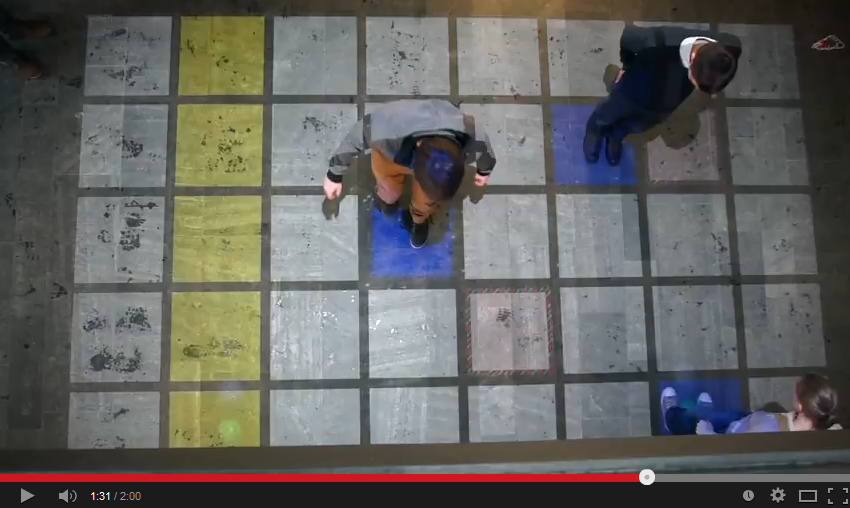
\includegraphics[width=0.9\textwidth]{images/showreel.png}
	\caption{Ausschnitt aus dem Showreel}
	\label{fig:showreel}
\end{figure}

Das Showreel soll für die Installation begeistern und Lust darauf machen diese selbst auszuprobieren. Dabei steht klar der spielerische, musikalische und gemeinschaftliche Aspekt im Vordergrund. Da die Installation musikalisch geprägt ist, wurde auf der Audioebene bewusst auf Sprachmitschnitte, Umgebungsgeräusche und Sprechertexte verzichtet. Es wurde besonderer Wert auf die Synchronisation der Musik und des Bildes gelegt, um eine bestmögliche Synthese der Sinneseindrücke zu erlangen. Auch das dramaturgische Konzept des Showreels lehnt sich an dem musikalischen Aufbau des verwendeten Stückes an. So sind bei Build-Ups vorwiegend Timelapse Aufnahmen zu sehen, die dann an Punkten des musikalischen Klimax von emotionalen und von Reaktionen geprägten Aufnahmen gebrochen werden. Bei solchen Aufnahmen wird ein breites Spektrum an Userreaktionen und Interaktionsmöglichkeiten gezeigt. Dabei wurden verschiedene Umgangsmöglichkeiten mit der Installation in den Fokus gerückt um die vielfältigen Möglichkeiten aufzuzeigen. Somit war es wichtig zu zeigen, welch unterschiedliche Formen der Joy-of-Use bei der Installation annimmt. Für einige Nutzer lag der Wettstreit mit anderen im Vordergrund, während andere mit der Erfassung verschiedener Gliedmaßen experimentierten. Wieder andere gingen sehr zögerlich und vorsichtig mit der Installation und waren überrascht über die musikalischen Folgen ihrer Interaktion. Andere Nutzer interagierten eher unbewusst mit der Installation indem sie einfach darüber liefen und On-the-fly interessante Tonfolgen kreierten, die weitere Zuschauer anlockten.